\documentclass[12pt, titlepage]{article}

\usepackage{fullpage}
\usepackage[round]{natbib}
\usepackage{multirow}
\usepackage{booktabs}
\usepackage{tabularx}
\usepackage{graphicx}
\usepackage{float}
\usepackage{hyperref}
\usepackage{ulem}
\usepackage{xcolor}
\hypersetup{
    colorlinks,
    citecolor=black,
    filecolor=black,
    linkcolor=red,
    urlcolor=blue
}
\usepackage[round]{natbib}

\newcounter{acnum}
\newcommand{\actheacnum}{AC\theacnum}
\newcommand{\acref}[1]{AC\ref{#1}}

\newcounter{ucnum}
\newcommand{\uctheucnum}{UC\theucnum}
\newcommand{\uref}[1]{UC\ref{#1}}

\newcounter{mnum}
\newcommand{\mthemnum}{M\themnum}
\newcommand{\mref}[1]{M\ref{#1}}

\title{SE 3XA3: Module Guide\\Super Refactored Mario Python}

\author{203, Abstract Connoisseurs 
		\\ David Jandric, jandricd
		\\ Daniel Noorduyn, noorduyd
		\\ Alexander Samaha, samahaa
}

\date{\today}

% \input{../../Comments}

\begin{document}

\maketitle

\pagenumbering{roman}
\tableofcontents
\listoftables
\listoffigures

\begin{table}[btp]
\caption{\bf Revision History}
\begin{tabularx}{\textwidth}{p{3cm}p{2cm}X}
\toprule {\bf Date} & {\bf Version} & {\bf Notes}\\
\midrule
13/03/20 & 1.0 & Initial Write of Modular Guide\\
\bottomrule
\end{tabularx}
\end{table}

\clearpage

\pagenumbering{arabic}

\section{Introduction}

\subsection{Overview}

Super Refactored Mario Bros is modeled after the original Super Mario Bros game from Nintendo. The goal of the project is to create an almost perfect clone of the original game, but make it open source. This would allow others to learn how to use the python library pygame. Additionally, the creator of the original code that this project is based on hasn't completed the game. Further, they have created some unorganized and quite amateur code which our team hopes to refactor into readable and understandable code. The team will also finish the game and add several key lacking features. \textcolor{red}{This document aims to translate the functional and non-functional requirements as seen in the \href{https://gitlab.cas.mcmaster.ca/jandric/super-refactored-mario-bros/-/blob/master/Doc/SRS/SRS.pdf}{\textcolor{red}{SRS}} into a direct programming scenario. This document outlines how behaviours desired in the SRS will be implemented into the code of the game. Our team has decided on a Main-Subroutine architecture which is how the following outlined modules are designed to interact with each other.}

\subsection{Scope}

The final version of Super Refactored Mario Bros will be a replica of the original Super Mario Bros game at its base functionality. It will be created solely using pygame. However, special features such as the multiplicity of power-ups or moving pipes or underground sections will not be implemented. This is because the goal of the team was to complete the base game and organize and/or rewrite the existing code.

\subsection{Purpose}

The purpose of this document is to provide a written, organized representation between the code design and the requirements. In a large program such as Super Refactored Mario Bros, there are many working parts that all need to work together seamlessly to create the desired program. As a result, this document will help the development team keep track of how the modules must interact and function. It also provides a map to future programmers who desire to add or change features to the open source game.

\section{Anticipated and Unlikely Changes} \label{SecChange}

This section lists possible changes to the system. According to the likeliness
of the change, the possible changes are classified into two
categories. Anticipated changes are listed in Section \ref{SecAchange}, and
unlikely changes are listed in Section \ref{SecUchange}.

\subsection{Anticipated Changes} \label{SecAchange}

Anticipated changes are the source of the information that is to be hidden
inside the modules. Ideally, changing one of the anticipated changes will only
require changing the one module that hides the associated decision. The approach
adapted here is called design for
change.

\begin{description}
\item[\refstepcounter{acnum} \actheacnum \label{acHardware}:] The specific hardware on which the software is running.
\item[\refstepcounter{acnum} \actheacnum \label{acCharacters}:] The amount and type of characters the user can choose from. 
\item[\refstepcounter{acnum} \actheacnum \label{acPower}:] The amount and type of power-ups from the item boxes.
\item[\refstepcounter{acnum} \actheacnum \label{acSpeed}:] The frame-rate of specific computers.
\item[\refstepcounter{acnum} \actheacnum \label{acRes}:] The resolution of different monitors.
\item[\refstepcounter{acnum} \actheacnum \label{acSound}:] The new sounds corresponding to any new features.
\end{description}

\subsection{Unlikely Changes} \label{SecUchange}

The module design should be as general as possible. However, a general system is
more complex. Sometimes this complexity is not necessary. Fixing some design
decisions at the system architecture stage can simplify the software design. If
these decision should later need to be changed, then many parts of the design
will potentially need to be modified. Hence, it is not intended that these
decisions will be changed.

\begin{description}
\item[\refstepcounter{ucnum} \uctheucnum \label{ucIO}:] The current and only input comes from specific keys on the user's keyboard. The keyboard allows the user to navigate menus and play the game. If this source of input were the change, the entire game would have to be re-designed.
\item[\refstepcounter{ucnum} \uctheucnum \label{ucWindow}:] The current game locks the size of the game window which results in a simple way to create and design new levels. If window resizing were to be implemented, a large section of the program would be heavily effected.
\end{description}

\section{Module Hierarchy} \label{SecMH}

This section provides an overview of the module design. Modules are summarized
in a hierarchy decomposed by secrets in Table \ref{TblMH}. The modules listed
below, which are leaves in the hierarchy tree, are the modules that will
actually be implemented.

\begin{description}
\item [\refstepcounter{mnum} \mthemnum \label{mGameController}:] \sout{Controller} \textcolor{red}{Game\_Controller}
\item [\refstepcounter{mnum} \mthemnum \label{mInput}:] Input
\item [\refstepcounter{mnum} \mthemnum \label{mMenu}:] Menu
\item [\refstepcounter{mnum} \mthemnum \label{mDashboard}:] Dashboard
\item [\refstepcounter{mnum} \mthemnum \label{mPause}:] Pause
\item [\refstepcounter{mnum} \mthemnum \label{mMario}:] Mario
\item [\refstepcounter{mnum} \mthemnum \label{mCamera}:] Camera
\item [\refstepcounter{mnum} \mthemnum \label{mGoomba}:] Goomba
\item [\refstepcounter{mnum} \mthemnum \label{mKoopa}:] Koopa
\item [\refstepcounter{mnum} \mthemnum \label{mVector2D}:] Vector2D
\item [\refstepcounter{mnum} \mthemnum \label{mSound}:] Sound\_Controller
\item [\refstepcounter{mnum} \mthemnum \label{mSpritesheet}:] Spritesheet
\item [\refstepcounter{mnum} \mthemnum \label{mCollider}:] Collider
\item [\refstepcounter{mnum} \mthemnum \label{mLevel}:] Level
\item [\sout{\refstepcounter{mnum} \mthemnum \label{mLevels}:}] \sout{Levels.json}
\item [\sout{\refstepcounter{mnum} \mthemnum \label{mSprites}:}] \sout{Sprites}
\item [\sout{\refstepcounter{mnum} \mthemnum \label{mSprite}:}] \sout{Sprite}
\item [\refstepcounter{mnum} \mthemnum \label{mEntityB}:] Entity\_Base
\item [\textcolor{red}{\refstepcounter{mnum} \mthemnum \label{mAnimation}:}] \textcolor{red}{Animation}
\item [\textcolor{red}{\refstepcounter{mnum} \mthemnum \label{mCoin}:}] \textcolor{red}{Coin}
\item [\textcolor{red}{\refstepcounter{mnum} \mthemnum \label{mItem}:}] \textcolor{red}{Item}
\item [\textcolor{red}{\refstepcounter{mnum} \mthemnum \label{mRandomBox}:}] \textcolor{red}{RandomBox}
\item [\textcolor{red}{\refstepcounter{mnum} \mthemnum \label{mMushroomItem}:}] \textcolor{red}{MushroomItem}
\item [\textcolor{red}{\refstepcounter{mnum} \mthemnum \label{mPowerUpBox}:}] \textcolor{red}{PowerUpBox}
\item [\textcolor{red}{\refstepcounter{mnum} \mthemnum \label{mEntityCollider}:}] \textcolor{red}{EntityCollider}
\item [\textcolor{red}{\refstepcounter{mnum} \mthemnum \label{mBounceTrait}:}] \textcolor{red}{BounceTrait}
\item [\textcolor{red}{\refstepcounter{mnum} \mthemnum \label{mGoTrait}:}] \textcolor{red}{GoTrait}
\item [\textcolor{red}{\refstepcounter{mnum} \mthemnum \label{mJumpTrait}:}] \textcolor{red}{JumpTrait}
\item [\textcolor{red}{\refstepcounter{mnum} \mthemnum \label{mLeftRightWalkTrait}:}] \textcolor{red}{LeftRightWalkTrait}
\item [\textcolor{red}{\refstepcounter{mnum} \mthemnum \label{mTile}:}] \textcolor{red}{Tile}
\end{description}

\begin{table}[h!]
\centering
\begin{tabular}{p{0.3\textwidth} p{0.6\textwidth}}
\toprule
\textbf{Level 1} & \textbf{Level 2}\\
\midrule

{Hardware-Hiding Module} & \sout{Controller} \textcolor{red}{Game\_Controller} \\
\midrule

\multirow{13}{0.3\textwidth}{Behaviour-Hiding Module} & Input\\
& Menu \\
& Dashboard\\
& Pause\\
& Mario\\
& Camera\\
& Goomba \\
& Koopa \\
& \textcolor{red}{Coin} \\
& \textcolor{red}{Item} \\
& \textcolor{red}{RandomBox} \\
& \textcolor{red}{MushroomItem} \\
& \textcolor{red}{PowerUpBox} \\
\midrule

\multirow{16}{0.3\textwidth}{Software Decision Module} & Vector2D\\
& Sound\_Controller\\
& SpriteSheet\\
& Collider\\
& Level\\
& \sout{Levels.json}\\
& \sout{Sprites} \\
& \sout{Sprite}\\
& \textcolor{red}{EntityBase} \\
& \textcolor{red}{Animation} \\
& \textcolor{red}{EntityCollider} \\
& \textcolor{red}{BounceTrait} \\
& \textcolor{red}{GoTrait} \\
& \textcolor{red}{JumpTrait} \\
& \textcolor{red}{LeftRightWalkTrait} \\
& \textcolor{red}{Tile} \\
\bottomrule

\end{tabular}
\caption{Module Hierarchy}
\label{TblMH}
\end{table}

\section{Connection Between Requirements and Design} \label{SecConnection}

The design of the system is intended to satisfy the requirements developed in
the \href{https://gitlab.cas.mcmaster.ca/jandric/super-refactored-mario-bros/-/blob/master/Doc/SRS/SRS.pdf}{SRS}. In this stage, the system is decomposed into modules. The connection between requirements and modules is listed in Table \ref{TblRT}.

\section{Module Decomposition} \label{SecMD}

Modules are decomposed according to the principle of ``information hiding''. The \emph{Secrets} field in a module
decomposition is a brief statement of the design decision hidden by the
module. The \emph{Services} field specifies \emph{what} the module will do
without documenting \emph{how} to do it. For each module, a suggestion for the
implementing software is given under the \emph{Implemented By} title. If the
entry is \emph{OS}, this means that the module is provided by the operating
system or by standard programming language libraries.  Also indicate if the
module will be implemented specifically for the software.

Only the leaf modules in the
hierarchy have to be implemented. If a dash (\emph{--}) is shown, this means
that the module is not a leaf and will not have to be implemented. Whether or
not this module is implemented depends on the programming language
selected.

\subsection{Hardware Hiding Modules (\mref{mGameController})}

\begin{description}
\item[Secrets:]The data structures and algorithms used to implement the virtual input and output
  hardware from the user's keyboard.
\item[Services:]Serves as a virtual hardware used by the rest of the
  system. This module provides the interface between the hardware and the
  software. So, the system can use it to display outputs or to accept inputs.
\item[Implemented By:] OS
\end{description}

\subsubsection{\textcolor{red}{Game\_Controller Module (\mref{mGameController})}}

\begin{description}
\item[\textcolor{red}{Secrets:}] \textcolor{red}{Process of starting the game, passing objects to others, and running the game.}
\item[\textcolor{red}{Services:}] \textcolor{red}{The main controller that initializes subroutines and organizes the functionality of the entire architecture.}
\item[\textcolor{red}{Implemented By:}] \textcolor{red}{Super Refactored Mario Bros}
\end{description}

\subsection{Behaviour-Hiding Module}

\begin{description}
\item[Secrets:] Required behaviours of the game elements.
\item[Services:]Includes programs that provide externally visible behaviour of
  the system as specified in the software requirements specification (SRS)
  documents. This module serves as a communication layer between the
  hardware-hiding module and the software decision module. The programs in this
  module will need to change if there are changes in the SRS.
\item[Implemented By:] Super Refactored Mario Bros
\end{description}

\subsubsection{Input Format Module (\mref{mInput})}

\begin{description}
\item[Secrets:]The format and structure of the input data.
\item[Services:]Converts the input data into the data structure used by the
  input parameters module.
\item[Implemented By:] Super Refactored Mario Bros
\end{description}

\subsubsection{Menu Module (\mref{mMenu})}

\begin{description}
\item[Secrets:] The format and structure of the game menu's items and graphics as well as links to other modules based on user selection.
\item[Services:] Displays the options on the game window and transfers the user to where they want to go in the game.
\item[Implemented By:] Super Refactored Mario Bros
\end{description}

\subsubsection{Dashboard Module (\mref{mDashboard})}

\begin{description}
\item[Secrets:] The formatting and gathering of the user's score, total collected coins, time left, and number of lives left.
\item[Services:] Displays the user's score, total collected coins, time left, and number of lives left in game.
\item[Implemented By:] Super Refactored Mario Bros
\end{description}

\subsubsection{Pause Module (\mref{mPause})}

\begin{description}
\item[Secrets:] The pausing of game play and creating a pause menu over top of the blurred current game window. Additionally it creates a link back to the main menu and manipulates game settings.
\item[Services:] Displays a menu that allows user to alter settings and provides a link back to the main menu.
\item[Implemented By:] Super Refactored Mario Bros
\end{description}

\subsubsection{Mario Module (\mref{mMario})}

\begin{description}
\item[Secrets:] How the character interacts with other objects in the game, such as enemies, blocks and coins.
\item[Services:] Provides the functionalities of the user playable character through the game.
\item[Implemented By:] Super Refactored Mario Bros
\end{description}

\subsubsection{Camera Module (\mref{mCamera})}

\begin{description}
\item[Secrets:] How the game camera pans and follows the user's character.
\item[Services:] Provides the driver to move the camera of the game as the user's character moves through the world.
\item[Implemented By:] Super Refactored Mario Bros
\end{description}

\subsubsection{Goomba Module (\mref{mGoomba})}

\begin{description}
\item[Secrets:] The function of the Goomba enemies \textcolor{red}{such as their movement and how they can be killed}.
\item[Services:] Allows the user to interact with an enemy, and gain points from their death.
\item[Implemented By:] Super Refactored Mario Bros
\end{description}

\subsubsection{Koopa Module (\mref{mKoopa})}

\begin{description}
\item[Secrets:] The function of the Koopa enemies \textcolor{red}{such as their movement, how they can be killed and their shell movement}.
\item[Services:] Allows the user to interact with an enemy, and gain points from their death.
\item[Implemented By:] Super Refactored Mario Bros
\end{description}

\subsubsection{\textcolor{red}{Coin Module (\mref{mCoin})}}

\begin{description}
\item[\textcolor{red}{Secrets:}] \textcolor{red}{Contains the coin animation (revolving) for static in level coins and how they can disappear.}
\item[\textcolor{red}{Services:}] \textcolor{red}{The user can interact with these coins to gain points.}
\item[\textcolor{red}{Implemented By:}] \textcolor{red}{Super Refactored Mario Bros}
\end{description}

\subsubsection{\textcolor{red}{Item Module (\mref{mItem})}}

\begin{description}
\item[\textcolor{red}{Secrets:}] \textcolor{red}{Contains the coin animation for appearing out of the random box and when/how the coins disappear.}
\item[\textcolor{red}{Services:}] \textcolor{red}{The user can interact with these coins to gain points.}
\item[\textcolor{red}{Implemented By:}] \textcolor{red}{Super Refactored Mario Bros}
\end{description}

\subsubsection{\textcolor{red}{RandomBox Module (\mref{mRandomBox})}}

\begin{description}
\item[\textcolor{red}{Secrets:}] \textcolor{red}{Contains the random box animation, and when the box is functional/non-functional.}
\item[\textcolor{red}{Services:}] \textcolor{red}{The user can interact with the box and gain points from getting coins from it.}
\item[\textcolor{red}{Implemented By:}] \textcolor{red}{Super Refactored Mario Bros}
\end{description}

\subsubsection{\textcolor{red}{MushroomItem Module (\mref{mMushroomItem})}}

\begin{description}
\item[\textcolor{red}{Secrets:}] \textcolor{red}{Contains the functions to make the mushrooms appear, move the mushroom, and disappear.}
\item[\textcolor{red}{Services:}] \textcolor{red}{The user can interact with these mushrooms to transform Mario from 'big Mario' to 'small Mario' and gain points.}
\item[\textcolor{red}{Implemented By:}] \textcolor{red}{Super Refactored Mario Bros}
\end{description}

\subsubsection{\textcolor{red}{PowerUpBox Module (\mref{mPowerUpBox})}}

\begin{description}
\item[\textcolor{red}{Secrets:}] \textcolor{red}{Contains the power-up box animation and when the box is functional/non-functional.}
\item[\textcolor{red}{Services:}] \textcolor{red}{The user can interact with the power-up box to get a mushroom to appear.}
\item[\textcolor{red}{Implemented By:}] \textcolor{red}{Super Refactored Mario Bros}
\end{description}

\subsection{Software Decision Module}

\begin{description}
\item[Secrets:] The design decision based on mathematical theorems, physical
  facts, or programming considerations. The secrets of this module are
  \emph{not} described in the SRS.
\item[Services:] Includes data structure and algorithms used in the system that
  do not provide direct interaction with the user. 
  % Changes in these modules are more likely to be motivated by a desire to
  % improve performance than by externally imposed changes.
\item[Implemented By:] Super Refactored Mario Bros
\end{description}

\subsubsection{Vector2D Module (\mref{mVector2D})}

\begin{description}
\item[Secrets:] The method of doing the vector addition, as well as calculation the magnitude of a vector.
\item[Services:] Uses vector addition in order to create new vectors for doing math with positions, velocities and accelerations. 
\item[Implemented By:] Super Refactored Mario Bros
\end{description}

\subsubsection{Sound\_Controller Module (\mref{mSound})}

\begin{description}
\item[Secrets:] The method of playing audio in the game for the user, which sounds are used and the channels over which he music and sounds will be played
\item[Services:] Provides functionality to play, stop and mute sounds or music.
\item[Implemented By:] Super Refactored Mario Bros
\end{description}

\subsubsection{SpriteSheet Module (\mref{mSpritesheet})}

\begin{description}
\item[Secrets:] Where and how the game accesses the various files to pull images from and create sprites
\item[Services:] Provides functionality to isolate an image to be used to create a sprite.
\item[Implemented By:] Super Refactored Mario Bros
\end{description}

\subsubsection{Collider Module (\mref{mCollider})}

\begin{description}
\item[Secrets:] How the game detects that two objects have overlapped and are in a collision state.
\item[Services:] Provides methods and functions to check positions to determine if a collision has occurred.
\item[Implemented By:] Super Refactored Mario Bros
\end{description}

\subsubsection{Level Module (\mref{mLevel})}

\begin{description}
\item[Secrets:] The method of which objects and entities in the game are spawned and placed in a level.
\item[Services:] Loads objects and entities from sprites and places them within the context of a level. 
\item[Implemented By:] Super Refactored Mario Bros
\end{description}

\subsubsection{\sout{Levels.json Module (\mref{mLevels})}}

\begin{description}
\item[\sout{Secrets:}] \sout{Contains the structure of every level as a combination of sprites.}
\item[\sout{Services:}] \sout{Used to create unique levels that the user can play.}
\item[\sout{Implemented By:}] \sout{Super Refactored Mario Bros}
\end{description}

\subsubsection{\sout{Sprites Module (\mref{mSprites})}}

\begin{description}
\item[\sout{Secrets:}] \sout{The method of which collections of sprites are loaded to be used in the game.}
\item[\sout{Services:}] \sout{Loads a collection of sprites to be used by the different entities and level building modules.}
\item[\sout{Implemented By:}] \sout{Super Refactored Mario Bros}
\end{description}

\subsubsection{\sout{Sprite Module (\mref{mSprite})}}

\begin{description}
\item[\sout{Secrets:}] \sout{The method of which the game draws a sprite.}
\item[\sout{Services:}] \sout{Provides functionalities to draw a sprite from an image to be used in the game.}
\item[\sout{Implemented By:}] \sout{Super Refactored Mario Bros}
\end{description}

\subsubsection{\sout{Sprite} \textcolor{red}{Entity Base} Module (\mref{mEntityB})}

\begin{description}
\item[Secrets:] The various fields that are general to all attributes in the game.
\item[Services:] Provides functionalities to update and access fields required of all attributes in the game.
\item[Implemented By:] Super Refactored Mario Bros
\end{description}

\subsubsection{\textcolor{red}{Animation Module (\mref{mAnimation})}}

\begin{description}
\item[\textcolor{red}{Secrets:}] \textcolor{red}{The images to be displayed and how they change over time.}
\item[\textcolor{red}{Services:}] \textcolor{red}{Provides animation functionality to any entities required by the game.}
\item[\textcolor{red}{Implemented By:}] \textcolor{red}{Super Refactored Mario Bros}
\end{description}

\subsubsection{\textcolor{red}{EntityCollider Module (\mref{mAEntityCollider})}}

\begin{description}
\item[\textcolor{red}{Secrets:}] \textcolor{red}{The methods for checking if two entities are colliding.}
\item[\textcolor{red}{Services:}] \textcolor{red}{Provides functionality to entities that can interact with other entities in the game.}
\item[\textcolor{red}{Implemented By:}] \textcolor{red}{Super Refactored Mario Bros}
\end{description}

\subsubsection{\textcolor{red}{BounceTrait Module (\mref{mBounceTrait})}}

\begin{description}
\item[\textcolor{red}{Secrets:}] \textcolor{red}{How this module updates an entities state.}
\item[\textcolor{red}{Services:}] \textcolor{red}{Gives entities a method for bouncing up.}
\item[\textcolor{red}{Implemented By:}] \textcolor{red}{Super Refactored Mario Bros}
\end{description}

\subsubsection{\textcolor{red}{GoTrait Module (\mref{mGoTrait})}}

\begin{description}
\item[\textcolor{red}{Secrets:}] \textcolor{red}{How this module updates an entities state and how it interacts with the user.}
\item[\textcolor{red}{Services:}] \textcolor{red}{Provides advanced movement functionality for an entity.}
\item[\textcolor{red}{Implemented By:}] \textcolor{red}{Super Refactored Mario Bros}
\end{description}

\subsubsection{\textcolor{red}{JumpTrait Module (\mref{mJumpTrait})}}

\begin{description}
\item[\textcolor{red}{Secrets:}] \textcolor{red}{How this module updates an entities state and how it interacts with the user.}
\item[\textcolor{red}{Services:}] \textcolor{red}{Provides jumping functionality to an entity.}
\item[\textcolor{red}{Implemented By:}] \textcolor{red}{Super Refactored Mario Bros}
\end{description}

\subsubsection{\textcolor{red}{LeftRightWalkTrait Module (\mref{mLeftRightWalkTrait})}}

\begin{description}
\item[\textcolor{red}{Secrets:}] \textcolor{red}{How this module updates an entities state.}
\item[\textcolor{red}{Services:}] \textcolor{red}{Provides simple horizontal movement to an entity.}
\item[\textcolor{red}{Implemented By:}] \textcolor{red}{Super Refactored Mario Bros}
\end{description}

\subsubsection{\textcolor{red}{Tile Module (\mref{mTile})}}

\begin{description}
\item[\textcolor{red}{Secrets:}] \textcolor{red}{How the module stores data.}
\item[\textcolor{red}{Services:}] \textcolor{red}{Provides a simple data class for representing a static object with an image.}
\item[\textcolor{red}{Implemented By:}] \textcolor{red}{Super Refactored Mario Bros}
\end{description}

\section{Traceability Matrix} \label{SecTM}

This section shows two traceability matrices: between the modules and the
requirements and between the modules and the anticipated changes.

% the table should use mref, the requirements should be named, use something
% like fref
\begin{table}[H]
\centering
\begin{tabular}{p{0.2\textwidth} p{0.6\textwidth}}
\toprule
\textbf{Req.} & \textbf{Modules}\\
\midrule
FR1 & \mref{mGameController}, \mref{mInput}, \mref{mMario}, \mref{mCollider}, \sout{\mref{mLevels}, \mref{mSprites}, \mref{mSprite}}, \textcolor{red}{\mref{mAnimation}, \mref{mEntityCollider}, \mref{mJumpTrait}}\\
FR2 & \mref{mGameController}, \mref{mInput}, \mref{mMario}, \mref{mCamera}, \mref{mCollider}, \sout{\mref{mLevels}, \mref{mSprites}, \mref{mSprite}}, \textcolor{red}{\mref{mAnimation}, \mref{mEntityCollider}}\\
\sout{FR3} & \sout{\mref{mGameController}, \mref{mInput}, \mref{mMario}, \mref{mCollider}, \mref{mLevels}, \mref{mSprites}, \mref{mSprite}}\\
FR4 & \mref{mGameController}, \mref{mInput}, \mref{mMario}, \mref{mCamera}, \mref{mCollider}, \sout{\mref{mLevels}, \mref{mSprites}, \mref{mSprite}}, \textcolor{red}{ \mref{mAnimation}, \mref{mEntityCollider}}\\
\sout{FR5} & \sout{\mref{mGameController}, \mref{mInput}, \mref{mMario}, \mref{mCamera}, \mref{mCollider}, \mref{mLevels}, \mref{mSprites}, \mref{mSprite}}\\
FR6 & \mref{mGameController}, \mref{mInput}, \mref{mMario}, \mref{mCamera}, \mref{mGoomba}, \mref{mCollider}, \sout{\mref{mLevels}, \mref{mSprites}, \mref{mSprite}}, \textcolor{red}{ \mref{mAnimation}, \mref{mEntityCollider}, \mref{mJumpTrait}, \mref{mLeftRightWalkTrait}}\\
FR7 & \mref{mGameController}, \mref{mInput}, \mref{mMario}, \mref{mCamera}, \mref{mKoopa}, \mref{mCollider}, \sout{\mref{mLevels}, \mref{mSprites}, \mref{mSprite}}, \mref{mEntityB}, \textcolor{red}{\mref{mAnimation}, \mref{mEntityCollider}, \mref{mGoTrait}, \mref{mJumpTrait}, \mref{mLeftRightWalkTrait}}\\
FR8 & \mref{mGameController}, \mref{mInput}, \mref{mMario}, \mref{mCamera}, \mref{mKoopa}, \mref{mCollider}, \sout{\mref{mLevels}, \mref{mSprites}, \mref{mSprite}}, \mref{mEntityB}, \textcolor{red}{\mref{mAnimation}, \mref{mEntityCollider}, \mref{mJumpTrait}, \mref{mBounceTrait}, \mref{mLeftRightWalkTrait}}\\
FR9 & \mref{mGameController}, \mref{mMario}, \mref{mCamera}, \mref{mGoomba}, \mref{mKoopa}, \mref{mCollider}, \sout{\mref{mLevels}, \mref{mSprites}, \mref{mSprite}}, \mref{mEntityB}, \textcolor{red}{\mref{mAnimation}, \mref{mEntityCollider}, \mref{mGoTrait}}\\
FR10 & \mref{mGameController}, \mref{mMario}, \textcolor{red}{\mref{mDashboard}} \\
FR11 & \mref{mGameController}, \mref{mDashboard}, \mref{mMario}\\
FR12 & \mref{mGameController}, \mref{mMenu}, \mref{mDashboard}, \mref{mMario}\\
FR13 & \mref{mGameController}, \mref{mLevel}, \sout{\mref{mLevels}}\\
FR14 & \mref{mGameController}, \mref{mDashboard}, \mref{mMario}\\
\textcolor{red}{FR15} & \textcolor{red}{\mref{mGameController}, \mref{mMario}, \mref{mMushroomItem}, \mref{mPowerUpBox}, \mref{mEntityCollider}, \mref{mJumpTrait}, \mref{mLeftRightWalkTrait}}\\
\textcolor{red}{FR16} & \textcolor{red}{\mref{mGameController}, \mref{mMario}, \mref{mMushroomItem}, \mref{mEntityCollider}, \mref{mLeftRightWalkTrait}}\\
\textcolor{red}{FR17} & \textcolor{red}{\mref{mGameController}, \mref{mMario}, \mref{mEntityCollider}, \mref{mLeftRightWalkTrait}}\\
\textcolor{red}{FR18} & \textcolor{red}{\mref{mGameController}, \mref{mDashboard}, \mref{mMario}, \mref{mItem}, \mref{mRandomBox}, \mref{mEntityCollider}, \mref{mJumpTrait}}\\
\textcolor{red}{FR19} & \textcolor{red}{\mref{mGameController}, \mref{mDashboard}, \mref{mMario}, \mref{mCoin}, \mref{mEntityCollider}}\\

\bottomrule
\end{tabular}
\caption{Trace Between Requirements and Modules}
\label{TblRT}
\end{table}

\begin{table}[H]
\centering
\begin{tabular}{p{0.2\textwidth} p{0.6\textwidth}}
\toprule
\textbf{AC} & \textbf{Modules}\\
\midrule
\acref{acHardware} & \mref{mGameController}, \mref{mInput}\\
\acref{acCharacters} & \mref{mMario}\\
\acref{acPower} & \mref{mMario}, \textcolor{red}{\mref{mPowerUpBox}}\\
\acref{acSpeed} & \mref{mGameController}\\
\acref{acRes} & \mref{mLevel}\\
\acref{acSound} & \mref{mSound}\\

\bottomrule
\end{tabular}
\caption{Trace Between Anticipated Changes and Modules}
\label{TblACT}
\end{table}

\section{Use Hierarchy Between Modules} \label{SecUse}

In this section, the uses hierarchy between modules is
provided. If two programs A and B that A {\em uses} B if
correct execution of B may be necessary for A to complete the task described in
its specification. That is, A {\em uses} B if there exist situations in which
the correct functioning of A depends upon the availability of a correct
implementation of B.  Figure \ref{FigUH} illustrates the use relation between
the modules. It can be seen that the graph is a directed acyclic graph
(DAG). Each level of the hierarchy offers a testable and usable subset of the
system, and modules in the higher level of the hierarchy are essentially simpler
because they use modules from the lower levels.

\textcolor{red}{OLD VERSION}
\begin{figure}[H]
\centering
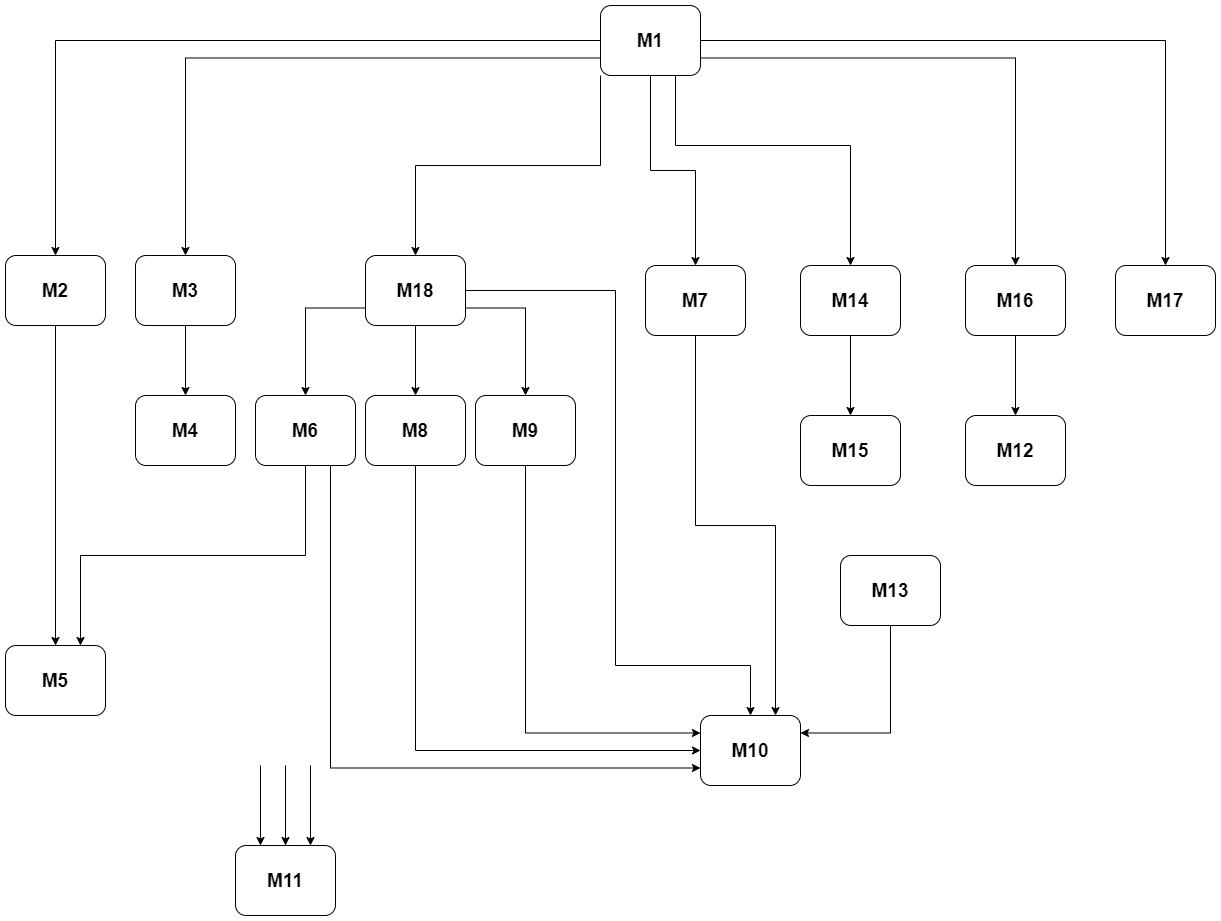
\includegraphics[width=0.7\textwidth]{UsesHierarchy.png}
\caption{Use hierarchy among modules}
\label{FigUH}
\end{figure}
\color{red}
\newpage
NEW VERSION
\begin{figure}[H]
\centering
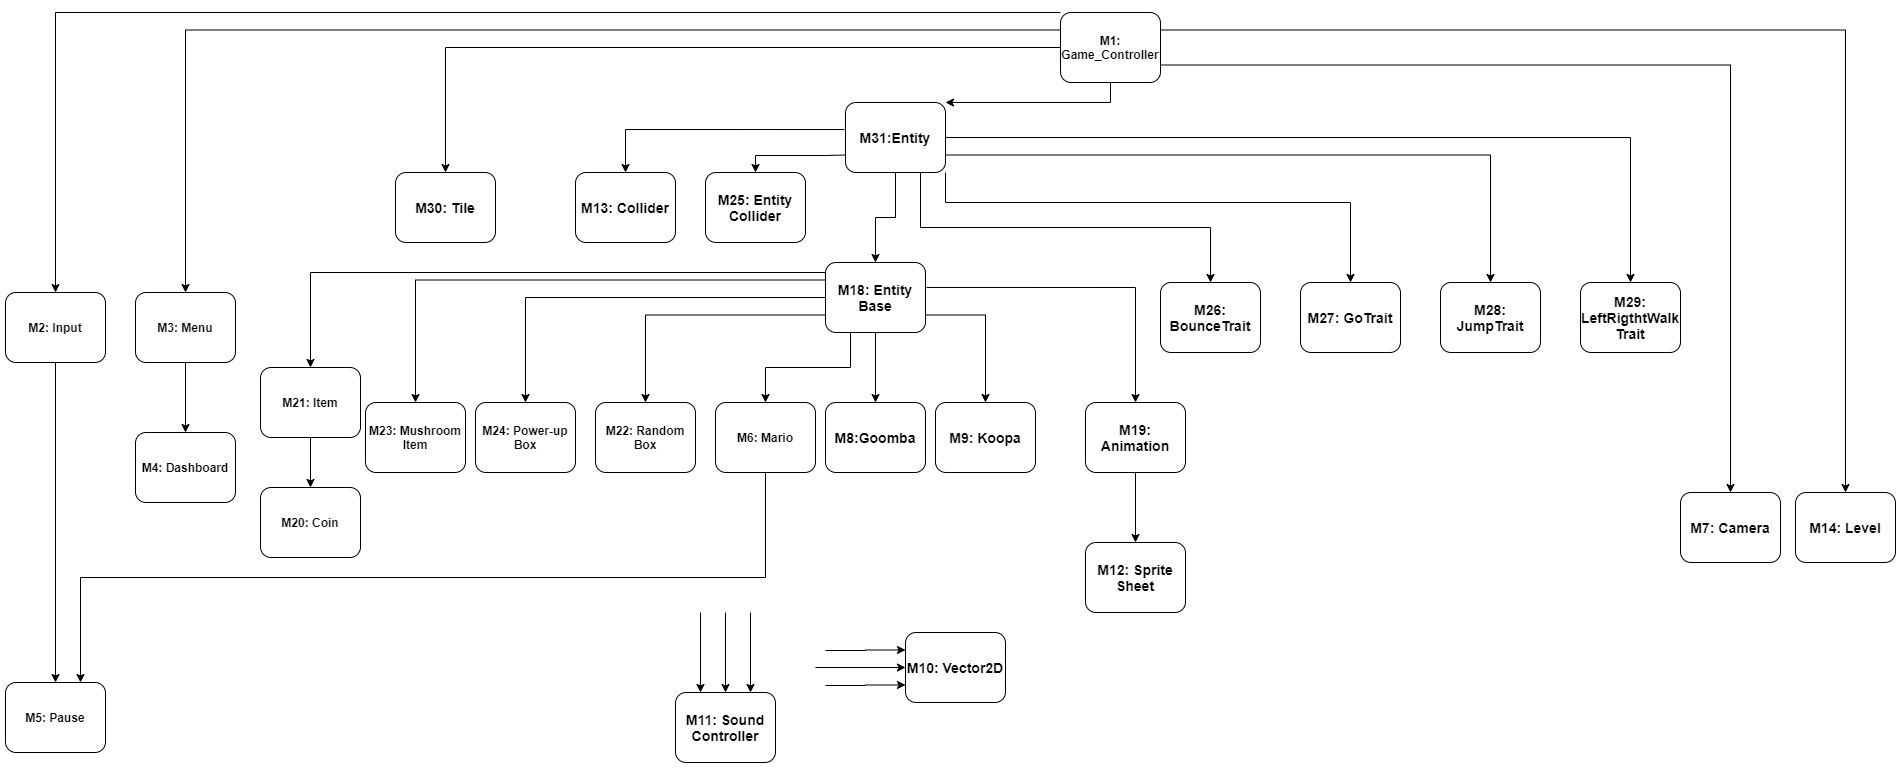
\includegraphics[width=1\textwidth]{Uses Hierarchy - 3XA3.png}
\caption{Use hierarchy among modules - Revision 1}
\label{FigUH2}
\end{figure}
\color{black}

%\section*{References}

\bibliographystyle {plainnat}
\bibliography {MG}

\end{document}